\documentclass[]{elsarticle} %review=doublespace preprint=single 5p=2 column
%%% Begin My package additions %%%%%%%%%%%%%%%%%%%

\usepackage[hyphens]{url}


\usepackage{graphicx}
%%%%%%%%%%%%%%%% end my additions to header

\usepackage[T1]{fontenc}
\usepackage{lmodern}
\usepackage{amssymb,amsmath}
% TODO: Currently lineno needs to be loaded after amsmath because of conflict
% https://github.com/latex-lineno/lineno/issues/5
\usepackage{lineno} % add
\usepackage{ifxetex,ifluatex}
\usepackage{fixltx2e} % provides \textsubscript
% use upquote if available, for straight quotes in verbatim environments
\IfFileExists{upquote.sty}{\usepackage{upquote}}{}
\ifnum 0\ifxetex 1\fi\ifluatex 1\fi=0 % if pdftex
  \usepackage[utf8]{inputenc}
\else % if luatex or xelatex
  \usepackage{fontspec}
  \ifxetex
    \usepackage{xltxtra,xunicode}
  \fi
  \defaultfontfeatures{Mapping=tex-text,Scale=MatchLowercase}
  \newcommand{\euro}{€}
\fi
% use microtype if available
\IfFileExists{microtype.sty}{\usepackage{microtype}}{}
\usepackage[margin=2cm]{geometry}
\usepackage[]{natbib}
\bibliographystyle{plainnat}

\usepackage{graphicx}
\ifxetex
  \usepackage[setpagesize=false, % page size defined by xetex
              unicode=false, % unicode breaks when used with xetex
              xetex]{hyperref}
\else
  \usepackage[unicode=true]{hyperref}
\fi
\hypersetup{breaklinks=true,
            bookmarks=true,
            pdfauthor={},
            pdftitle={Proyecto Registros Tratamiento de Datos Curso 2024-2025},
            colorlinks=false,
            urlcolor=blue,
            linkcolor=magenta,
            pdfborder={0 0 0}}

\setcounter{secnumdepth}{0}
% Pandoc toggle for numbering sections (defaults to be off)
\setcounter{secnumdepth}{0}

% Pandoc syntax highlighting
\usepackage{color}
\usepackage{fancyvrb}
\newcommand{\VerbBar}{|}
\newcommand{\VERB}{\Verb[commandchars=\\\{\}]}
\DefineVerbatimEnvironment{Highlighting}{Verbatim}{commandchars=\\\{\}}
% Add ',fontsize=\small' for more characters per line
\usepackage{framed}
\definecolor{shadecolor}{RGB}{248,248,248}
\newenvironment{Shaded}{\begin{snugshade}}{\end{snugshade}}
\newcommand{\AlertTok}[1]{\textcolor[rgb]{0.94,0.16,0.16}{#1}}
\newcommand{\AnnotationTok}[1]{\textcolor[rgb]{0.56,0.35,0.01}{\textbf{\textit{#1}}}}
\newcommand{\AttributeTok}[1]{\textcolor[rgb]{0.13,0.29,0.53}{#1}}
\newcommand{\BaseNTok}[1]{\textcolor[rgb]{0.00,0.00,0.81}{#1}}
\newcommand{\BuiltInTok}[1]{#1}
\newcommand{\CharTok}[1]{\textcolor[rgb]{0.31,0.60,0.02}{#1}}
\newcommand{\CommentTok}[1]{\textcolor[rgb]{0.56,0.35,0.01}{\textit{#1}}}
\newcommand{\CommentVarTok}[1]{\textcolor[rgb]{0.56,0.35,0.01}{\textbf{\textit{#1}}}}
\newcommand{\ConstantTok}[1]{\textcolor[rgb]{0.56,0.35,0.01}{#1}}
\newcommand{\ControlFlowTok}[1]{\textcolor[rgb]{0.13,0.29,0.53}{\textbf{#1}}}
\newcommand{\DataTypeTok}[1]{\textcolor[rgb]{0.13,0.29,0.53}{#1}}
\newcommand{\DecValTok}[1]{\textcolor[rgb]{0.00,0.00,0.81}{#1}}
\newcommand{\DocumentationTok}[1]{\textcolor[rgb]{0.56,0.35,0.01}{\textbf{\textit{#1}}}}
\newcommand{\ErrorTok}[1]{\textcolor[rgb]{0.64,0.00,0.00}{\textbf{#1}}}
\newcommand{\ExtensionTok}[1]{#1}
\newcommand{\FloatTok}[1]{\textcolor[rgb]{0.00,0.00,0.81}{#1}}
\newcommand{\FunctionTok}[1]{\textcolor[rgb]{0.13,0.29,0.53}{\textbf{#1}}}
\newcommand{\ImportTok}[1]{#1}
\newcommand{\InformationTok}[1]{\textcolor[rgb]{0.56,0.35,0.01}{\textbf{\textit{#1}}}}
\newcommand{\KeywordTok}[1]{\textcolor[rgb]{0.13,0.29,0.53}{\textbf{#1}}}
\newcommand{\NormalTok}[1]{#1}
\newcommand{\OperatorTok}[1]{\textcolor[rgb]{0.81,0.36,0.00}{\textbf{#1}}}
\newcommand{\OtherTok}[1]{\textcolor[rgb]{0.56,0.35,0.01}{#1}}
\newcommand{\PreprocessorTok}[1]{\textcolor[rgb]{0.56,0.35,0.01}{\textit{#1}}}
\newcommand{\RegionMarkerTok}[1]{#1}
\newcommand{\SpecialCharTok}[1]{\textcolor[rgb]{0.81,0.36,0.00}{\textbf{#1}}}
\newcommand{\SpecialStringTok}[1]{\textcolor[rgb]{0.31,0.60,0.02}{#1}}
\newcommand{\StringTok}[1]{\textcolor[rgb]{0.31,0.60,0.02}{#1}}
\newcommand{\VariableTok}[1]{\textcolor[rgb]{0.00,0.00,0.00}{#1}}
\newcommand{\VerbatimStringTok}[1]{\textcolor[rgb]{0.31,0.60,0.02}{#1}}
\newcommand{\WarningTok}[1]{\textcolor[rgb]{0.56,0.35,0.01}{\textbf{\textit{#1}}}}

% tightlist command for lists without linebreak
\providecommand{\tightlist}{%
  \setlength{\itemsep}{0pt}\setlength{\parskip}{0pt}}




\newcounter{none}
\usepackage{booktabs}
\usepackage{longtable}
\providecommand{\pandocbounded}[1]{#1}
\usepackage{pdflscape}
\usepackage{booktabs}
\usepackage{longtable}
\usepackage{array}
\usepackage{multirow}
\usepackage{wrapfig}
\usepackage{float}
\usepackage{colortbl}
\usepackage{pdflscape}
\usepackage{tabu}
\usepackage{threeparttable}
\usepackage{threeparttablex}
\usepackage[normalem]{ulem}
\usepackage{makecell}
\usepackage{xcolor}



\begin{document}


\begin{frontmatter}

  \title{Proyecto Registros Tratamiento de Datos Curso 2024-2025}
    \author[a]{Aleix Cebrián Valero%
  %
  }
  
    \author[b]{Carlos Albiach Melgar%
  %
  }
  
      \affiliation[a]{leutnant@fh-muenster.de}
    \affiliation[b]{caralmel@alumni.uv.es}
    \cortext[cor1]{Corresponding author}
  
  \begin{abstract}
  Este proyecto tiene como objetivo hallar información a partir de un
  archivo CSV con los registros de los usuarios de TD 2024-2025.

  \emph{Nota: Todos los miembros han participado equitativamente en el
  trabajo.}
  \end{abstract}
  
 \end{frontmatter}

\newpage

\section{Componentes del fichero}\label{componentes-del-fichero}

Hay un total de 26 compnenetes en el fichero.

\begin{Shaded}
\begin{Highlighting}[]
\NormalTok{type }\OtherTok{\textless{}{-}} \FunctionTok{as.character}\NormalTok{(}\FunctionTok{unique}\NormalTok{(df\_users}\SpecialCharTok{$}\NormalTok{Componente))}
\NormalTok{knitr}\SpecialCharTok{::}\FunctionTok{kable}\NormalTok{(rticles}\SpecialCharTok{::}\FunctionTok{string\_to\_table}\NormalTok{(type, }\DecValTok{3}\NormalTok{), }
             \AttributeTok{col.names =} \ConstantTok{NULL}\NormalTok{, }\AttributeTok{format =} \StringTok{"latex"}\NormalTok{, }\AttributeTok{booktab =} \ConstantTok{TRUE}\NormalTok{, }
             \AttributeTok{caption =} \StringTok{"Componentes del fichero."}\NormalTok{)}
\end{Highlighting}
\end{Shaded}

\begin{table}

\caption{\label{tab:tab_componentes}Componentes del fichero.}
\centering
\begin{tabular}[t]{lll}
\toprule
Registros & URL & Informe general\\
Actividad del curso & Encuesta & Diálogo\\
Sistema & Foro & Wooclap\\
Tarea & Informe del calificador & Hoja de cálculo Excel\\
Cuestionario & Papelera de reciclaje & Herramienta Externa\\
\addlinespace
Carpeta & Aplicación de Actas (XSLX) & Entregas de texto en línea\\
Asistencia & Vista Simple & Participación en el curso\\
Recurso & Comentarios de la entrega & Taller\\
Usuario & Archivos enviados & \\
\bottomrule
\end{tabular}
\end{table}

Como se puede observar en la Tabla \ref{tab:tab_componentes}, hay 26
componentes.

\section{Usuarios más activos}\label{usuarios-muxe1s-activos}

Vamos a ver que usuario ha sido el que más veces se ha registrado.

\begin{verbatim}
## U0001 
##  6932
\end{verbatim}

\begin{figure}

{\centering 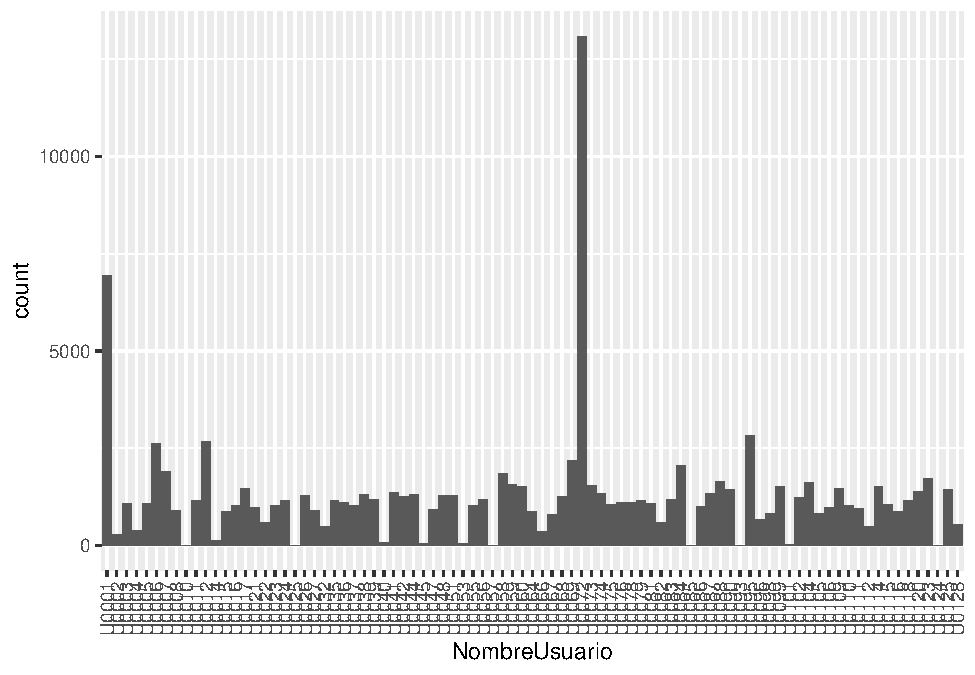
\includegraphics[width=1\linewidth]{ProyectoTD2026_files/figure-latex/fig1-1} 

}

\caption{A figure added with a code chunk.\label{fig:fig1}, echo = FALSE, message=FALSE, warning=FALSE, results='hide'}\label{fig:fig1}
\end{figure}

Como podemos ver en la Figura \ref{fig:fig1}, hay un tipo to rayao.

\section{Usuarios más activos 2}\label{usuarios-muxe1s-activos-2}

Vamos a ver que usuario ha sido el que más veces se ha registrado. I

\par

\begin{landscape}


```
\section{Usuarios más activos}
```

\begin{figure}

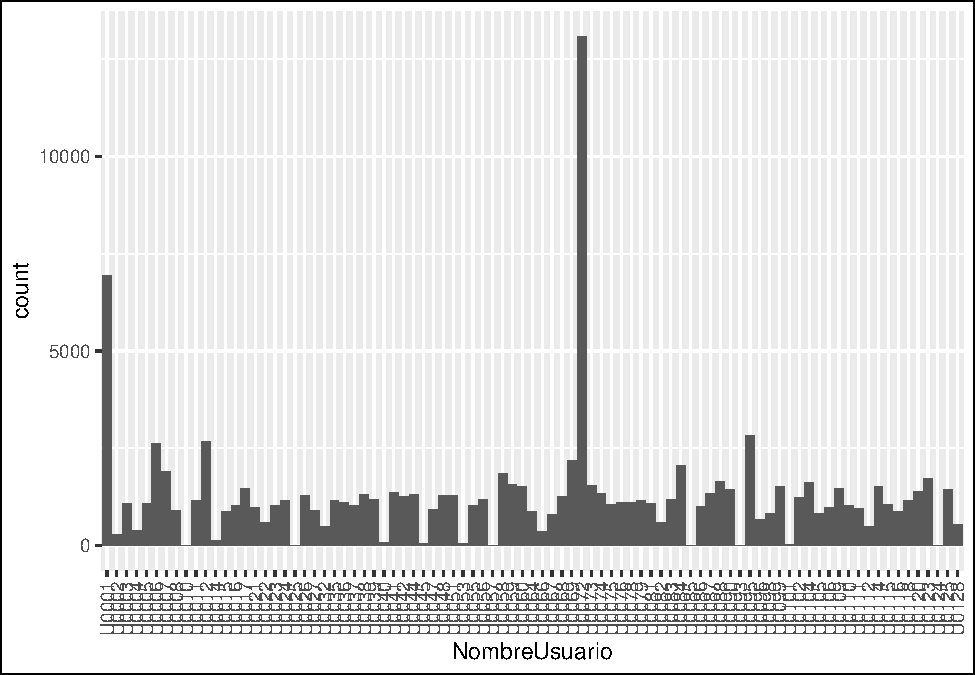
\includegraphics[width=1\linewidth]{ProyectoTD2026_files/figure-latex/fig3-1} \hfill{}

\caption{\label{fig2}Bar plot horizontal!!.}\label{fig:fig3}
\end{figure}

\end{landscape}

Como podemos ver en la Figura \ref{fig:fig3}, hay un tipo to rayao.

\section{Mes con más registros}\label{mes-con-muxe1s-registros}

Los meses en los que más registros han habido

\begin{figure}

{\centering 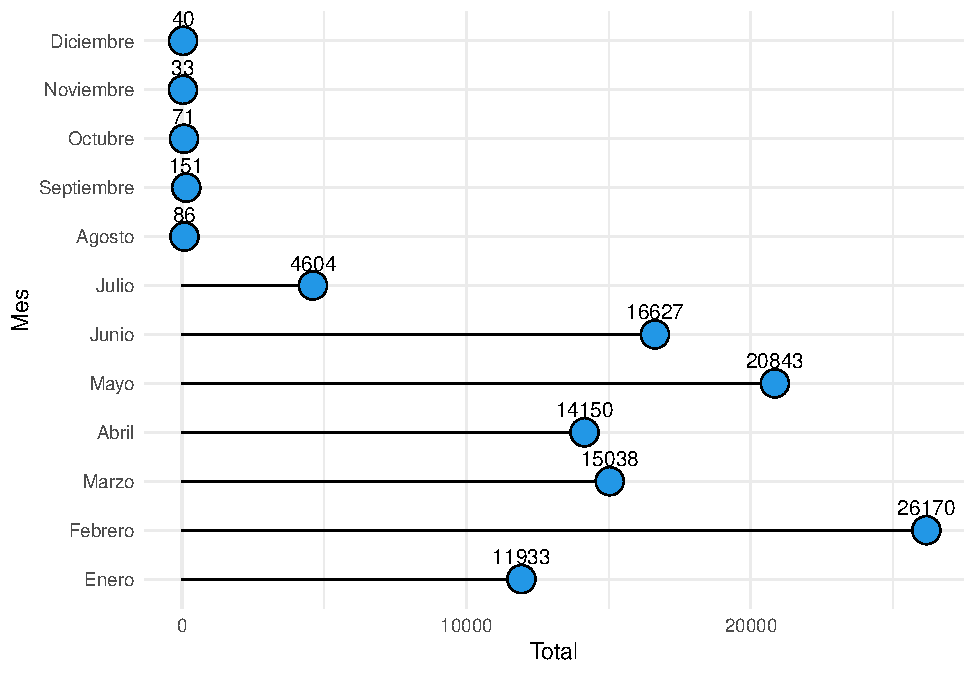
\includegraphics[width=1\linewidth]{ProyectoTD2026_files/figure-latex/fig4-1} 

}

\caption{\label{fig2}Bar plot horizontal!!.}\label{fig:fig4}
\end{figure}

\section{Contexto con más
registros}\label{contexto-con-muxe1s-registros}

Los contextos más visitados son:

\begin{Shaded}
\begin{Highlighting}[]
\FunctionTok{library}\NormalTok{(dplyr)}
\NormalTok{df\_users }\SpecialCharTok{\%\textgreater{}\%} \FunctionTok{group\_by}\NormalTok{(ContextoEvento) }\SpecialCharTok{\%\textgreater{}\%} \FunctionTok{count}\NormalTok{() }\SpecialCharTok{\%\textgreater{}\%} \FunctionTok{filter}\NormalTok{(n}\SpecialCharTok{\textless{}}\DecValTok{30000}\NormalTok{)}
\end{Highlighting}
\end{Shaded}

\begin{verbatim}
## # A tibble: 174 x 2
## # Groups:   ContextoEvento [174]
##    ContextoEvento                                   n
##    <chr>                                        <int>
##  1 Archivo: Alumnos23-24                            4
##  2 Archivo: Alumnos24-25                           26
##  3 Archivo: Cheatsheets de uso frecuente           85
##  4 Archivo: Comentarios entrega preliminar 2025    49
##  5 Archivo: Cómo preparar una presentación         80
##  6 Archivo: Datos Proyecto 2C                       1
##  7 Archivo: Ejemplo Wordclouds                     50
##  8 Archivo: Ejercicio correos                      96
##  9 Archivo: Ejercicio. Logs conexiones             55
## 10 Archivo: EntregaIntermediateR24-25              26
## # i 164 more rows
\end{verbatim}

\begin{Shaded}
\begin{Highlighting}[]
\FunctionTok{ggplot}\NormalTok{(df\_users }\SpecialCharTok{\%\textgreater{}\%} \FunctionTok{group\_by}\NormalTok{(ContextoEvento) }\SpecialCharTok{\%\textgreater{}\%} \FunctionTok{count}\NormalTok{() }\SpecialCharTok{\%\textgreater{}\%} \FunctionTok{filter}\NormalTok{(n}\SpecialCharTok{\textless{}}\DecValTok{30000} \SpecialCharTok{\&}\NormalTok{ n }\SpecialCharTok{\textgreater{}} \DecValTok{500}\NormalTok{), }\FunctionTok{aes}\NormalTok{(}\AttributeTok{x =}\NormalTok{ ContextoEvento, }\AttributeTok{y =}\NormalTok{ n)) }\SpecialCharTok{+} \FunctionTok{geom\_col}\NormalTok{() }\SpecialCharTok{+}
  \FunctionTok{theme}\NormalTok{(}\AttributeTok{axis.text.x =} \FunctionTok{element\_text}\NormalTok{(}\AttributeTok{angle =} \DecValTok{90}\NormalTok{, }\AttributeTok{vjust =} \FloatTok{0.5}\NormalTok{, }\AttributeTok{hjust =} \DecValTok{1}\NormalTok{), }\AttributeTok{plot.background =} \FunctionTok{element\_rect}\NormalTok{(}\AttributeTok{color =} \StringTok{"black"}\NormalTok{))}
\end{Highlighting}
\end{Shaded}

\pandocbounded{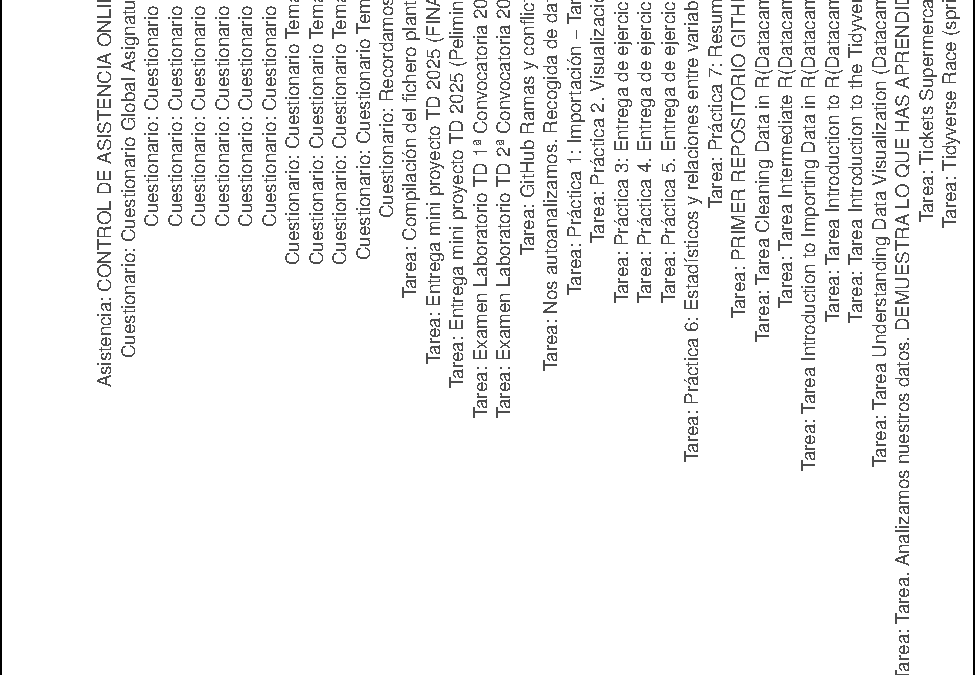
\includegraphics[keepaspectratio]{ProyectoTD2026_files/figure-latex/unnamed-chunk-3-1.pdf}}

\begin{Shaded}
\begin{Highlighting}[]
\CommentTok{\# Todos los componentes}
\FunctionTok{library}\NormalTok{(stringr)}

\CommentTok{\#df\_teacher \textless{}{-} df\_users \%\textgreater{}\% filter(NombreUsuario == "U0072")}

\FunctionTok{ggplot}\NormalTok{(df\_users, }\FunctionTok{aes}\NormalTok{(}\AttributeTok{x =}\NormalTok{ Componente)) }\SpecialCharTok{+} \FunctionTok{geom\_bar}\NormalTok{()}\SpecialCharTok{+}
  \FunctionTok{theme}\NormalTok{(}\AttributeTok{axis.text.x =} \FunctionTok{element\_text}\NormalTok{(}\AttributeTok{angle =} \DecValTok{90}\NormalTok{, }\AttributeTok{vjust =} \FloatTok{0.5}\NormalTok{, }\AttributeTok{hjust =} \DecValTok{1}\NormalTok{), }\AttributeTok{plot.background =} \FunctionTok{element\_rect}\NormalTok{(}\AttributeTok{color =} \StringTok{"black"}\NormalTok{))}
\end{Highlighting}
\end{Shaded}

\pandocbounded{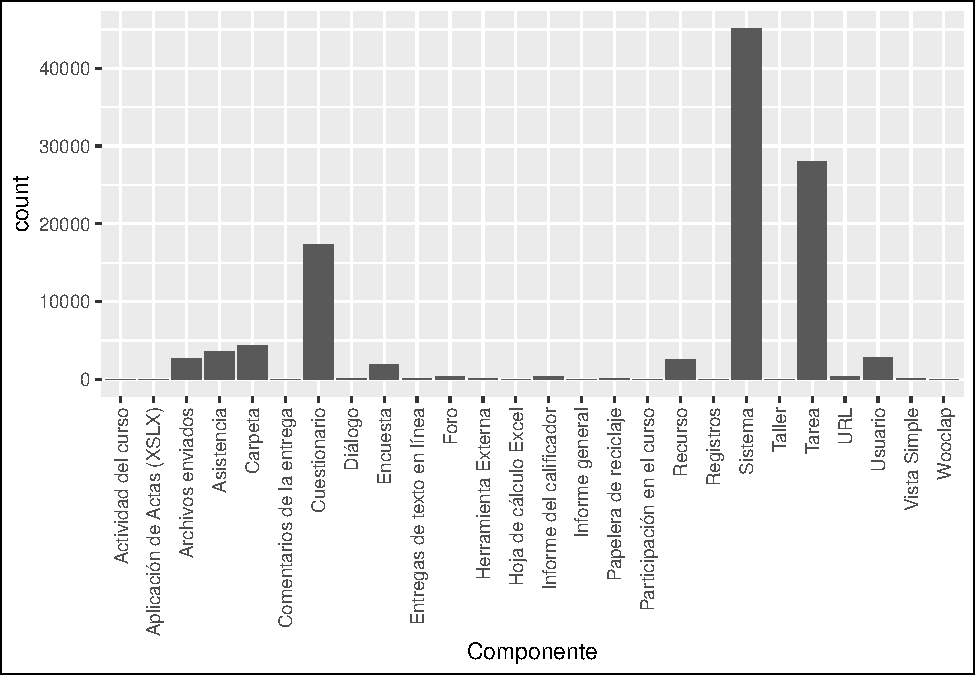
\includegraphics[keepaspectratio]{ProyectoTD2026_files/figure-latex/unnamed-chunk-4-1.pdf}}

\begin{Shaded}
\begin{Highlighting}[]
\DocumentationTok{\#\# Todos los cuestionarios}
\FunctionTok{ggplot}\NormalTok{(df\_users }\SpecialCharTok{\%\textgreater{}\%} \FunctionTok{filter}\NormalTok{(Componente }\SpecialCharTok{==} \StringTok{"Cuestionario"}\NormalTok{), }\FunctionTok{aes}\NormalTok{(}\AttributeTok{x =}\NormalTok{ ContextoEvento)) }\SpecialCharTok{+} \FunctionTok{geom\_bar}\NormalTok{()}\SpecialCharTok{+}
  \FunctionTok{theme}\NormalTok{(}\AttributeTok{axis.text.x =} \FunctionTok{element\_text}\NormalTok{(}\AttributeTok{angle =} \DecValTok{90}\NormalTok{, }\AttributeTok{vjust =} \FloatTok{0.5}\NormalTok{, }\AttributeTok{hjust =} \DecValTok{1}\NormalTok{), }\AttributeTok{plot.background =} \FunctionTok{element\_rect}\NormalTok{(}\AttributeTok{color =} \StringTok{"black"}\NormalTok{))}
\end{Highlighting}
\end{Shaded}

\pandocbounded{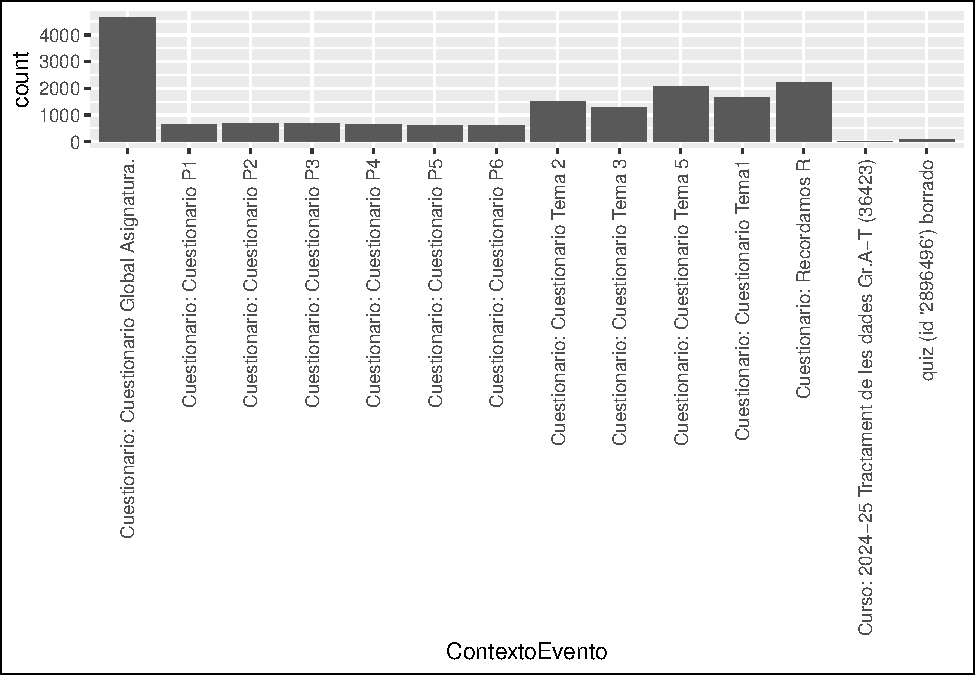
\includegraphics[keepaspectratio]{ProyectoTD2026_files/figure-latex/unnamed-chunk-4-2.pdf}}

\begin{Shaded}
\begin{Highlighting}[]
\FunctionTok{nrow}\NormalTok{(df\_users }\SpecialCharTok{\%\textgreater{}\%} \FunctionTok{filter}\NormalTok{(Componente }\SpecialCharTok{==} \StringTok{"Cuestionario"}\NormalTok{) }\SpecialCharTok{\%\textgreater{}\%} \FunctionTok{distinct}\NormalTok{(ContextoEvento)) }\CommentTok{\# Cantidad de cuestionarios}
\end{Highlighting}
\end{Shaded}

\begin{verbatim}
## [1] 14
\end{verbatim}

\begin{Shaded}
\begin{Highlighting}[]
\DocumentationTok{\#\# Todas las tareas}
\FunctionTok{ggplot}\NormalTok{(df\_users }\SpecialCharTok{\%\textgreater{}\%} \FunctionTok{filter}\NormalTok{(Componente }\SpecialCharTok{==} \StringTok{"Tarea"}\NormalTok{), }\FunctionTok{aes}\NormalTok{(}\AttributeTok{x =}\NormalTok{ ContextoEvento)) }\SpecialCharTok{+} \FunctionTok{geom\_bar}\NormalTok{()}\SpecialCharTok{+}
  \FunctionTok{theme}\NormalTok{(}\AttributeTok{axis.text.x =} \FunctionTok{element\_text}\NormalTok{(}\AttributeTok{angle =} \DecValTok{90}\NormalTok{, }\AttributeTok{vjust =} \FloatTok{0.5}\NormalTok{, }\AttributeTok{hjust =} \DecValTok{1}\NormalTok{), }\AttributeTok{plot.background =} \FunctionTok{element\_rect}\NormalTok{(}\AttributeTok{color =} \StringTok{"black"}\NormalTok{))}
\end{Highlighting}
\end{Shaded}

\pandocbounded{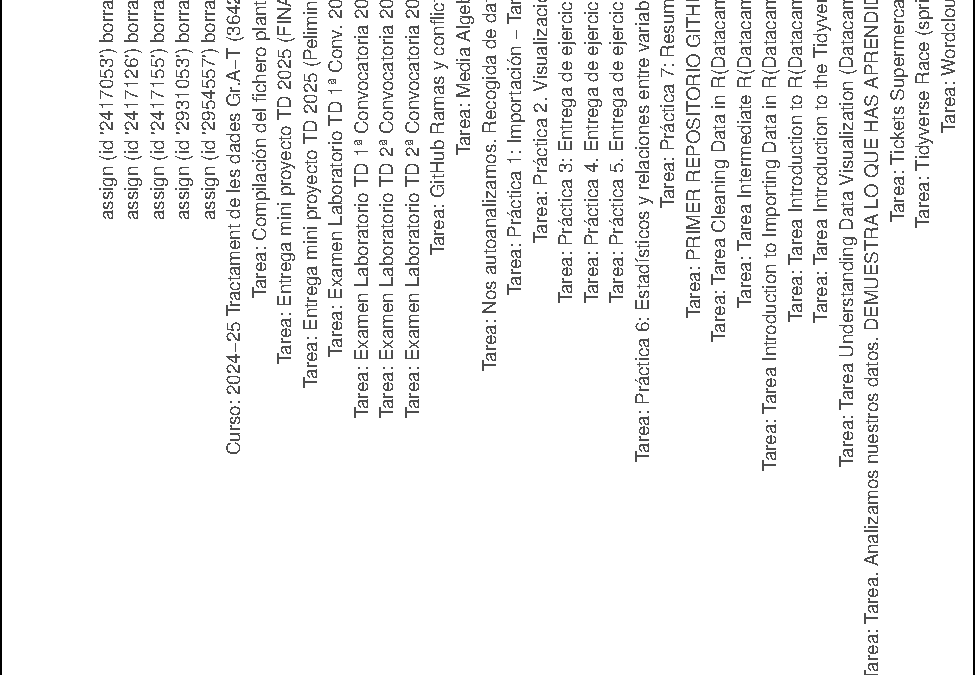
\includegraphics[keepaspectratio]{ProyectoTD2026_files/figure-latex/unnamed-chunk-4-3.pdf}}

\begin{Shaded}
\begin{Highlighting}[]
\FunctionTok{nrow}\NormalTok{(df\_users }\SpecialCharTok{\%\textgreater{}\%} \FunctionTok{filter}\NormalTok{(Componente }\SpecialCharTok{==} \StringTok{"Tarea"}\NormalTok{) }\SpecialCharTok{\%\textgreater{}\%} \FunctionTok{distinct}\NormalTok{(ContextoEvento)) }\CommentTok{\# Cantidad de tareas}
\end{Highlighting}
\end{Shaded}

\begin{verbatim}
## [1] 34
\end{verbatim}

\section{Usuarios sin
retroalimentación}\label{usuarios-sin-retroalimentaciuxf3n}

\begin{Shaded}
\begin{Highlighting}[]
\CommentTok{\#table((df\_users \%\textgreater{}\% filter(!is.na(UsuarioAfectado))) == (df\_users \%\textgreater{}\% filter(!is.na(UsuarioAfectado))))}

\NormalTok{df\_users\_usuario\_afectado }\OtherTok{\textless{}{-}}\NormalTok{ df\_users }\SpecialCharTok{\%\textgreater{}\%} \FunctionTok{filter}\NormalTok{(}\SpecialCharTok{!}\FunctionTok{is.na}\NormalTok{(UsuarioAfectado) }\SpecialCharTok{\&}\NormalTok{ UsuarioAfectado }\SpecialCharTok{!=}\NormalTok{ NombreUsuario)}

\FunctionTok{unique}\NormalTok{(df\_users\_usuario\_afectado}\SpecialCharTok{$}\NormalTok{NombreEvento)}
\end{Highlighting}
\end{Shaded}

\begin{verbatim}
##  [1] "Perfil de usuario visto"                
##  [2] "Formulario de calificaciones visto"     
##  [3] "Informe de notas de usuario visto"      
##  [4] "Usuario calificado"                     
##  [5] "Se ha calificado el envío."             
##  [6] "Calificación borrada"                   
##  [7] "Intento abandonado"                     
##  [8] "Tiempo límite del cuestionario excedido"
##  [9] "Usuario desmatriculado del curso"       
## [10] "Miembro del grupo eliminado"            
## [11] "Rol sin asignar"                        
## [12] "Retroalimentación vista"                
## [13] "Informe de registro visualizado"        
## [14] "Rol asignado"                           
## [15] "Usuario matriculado en el curso"        
## [16] "Intento enviado"                        
## [17] "Informe del usuario visualizado"        
## [18] "Miembro del grupo añadido"              
## [19] "Intento de cuestionario recalificado"
\end{verbatim}

\begin{Shaded}
\begin{Highlighting}[]
\FunctionTok{unique}\NormalTok{((df\_users\_usuario\_afectado }\SpecialCharTok{\%\textgreater{}\%} \FunctionTok{filter}\NormalTok{(NombreEvento }\SpecialCharTok{==} \StringTok{"Usuario matriculado en el curso"}\NormalTok{))}\SpecialCharTok{$}\NormalTok{UsuarioAfectado)}
\end{Highlighting}
\end{Shaded}

\begin{verbatim}
##   [1] "U0082" "U0098" "U0070" "U0053" "U0128" "U0120" "U0095" "U0057" "U0049"
##  [10] "U0030" "U0119" "U0062" "U0089" "U0100" "U0103" "U0050" "U0034" "U0029"
##  [19] "U0093" "U0076" "U0073" "U0123" "U0047" "U0032" "U0060" "U0069" "U0023"
##  [28] "U0026" "U0078" "U0020" "U0036" "U0067" "U0108" "U0012" "U0009" "U0075"
##  [37] "U0105" "U0086" "U0048" "U0043" "U0035" "U0115" "U0112" "U0083" "U0042"
##  [46] "U0015" "U0041" "U0096" "U0025" "U0005" "U0074" "U0018" "U0058" "U0022"
##  [55] "U0106" "U0038" "U0016" "U0064" "U0013" "U0084" "U0055" "U0021" "U0045"
##  [64] "U0031" "U0044" "U0079" "U0081" "U0027" "U0090" "U0085" "U0006" "U0104"
##  [73] "U0088" "U0080" "U0117" "U0065" "U0114" "U0111" "U0037" "U0126" "U0118"
##  [82] "U0061" "U0046" "U0039" "U0107" "U0028" "U0094" "U0004" "U0116" "U0019"
##  [91] "U0051" "U0121" "U0097" "U0087" "U0024" "U0099" "U0071" "U0110" "U0068"
## [100] "U0091" "U0033" "U0014" "U0052" "U0007" "U0003" "U0122" "U0092" "U0063"
## [109] "U0072" "U0066" "U0010" "U0127" "U0056" "U0102" "U0054" "U0077" "U0113"
## [118] "U0017" "U0109" "U0011" "U0124" "U0059" "U0008"
\end{verbatim}

\begin{Shaded}
\begin{Highlighting}[]
\FunctionTok{length}\NormalTok{(}\FunctionTok{unique}\NormalTok{(df\_users}\SpecialCharTok{$}\NormalTok{UsuarioAfectado))}
\end{Highlighting}
\end{Shaded}

\begin{verbatim}
## [1] 125
\end{verbatim}

Parece que el usuario U0071 no ha hecho nada en todo el curso, y U0072
sha sido desmatriculado.


\end{document}
